\chapter{Methodology}
\label{cap:method}

\intro{In this chapter, we will present the methodology used to develop the proposed solution. The chapter is divided into two sections: architecture, and implementation. The architecture section will present the proposed solution's architecture for the chosen cloud providers, while the implementation section will detail the steps taken to implement the solution.
}\\


\section{Architecture}
\label{sec:architecture}

\begin{figure}[htbp]
    \centering
    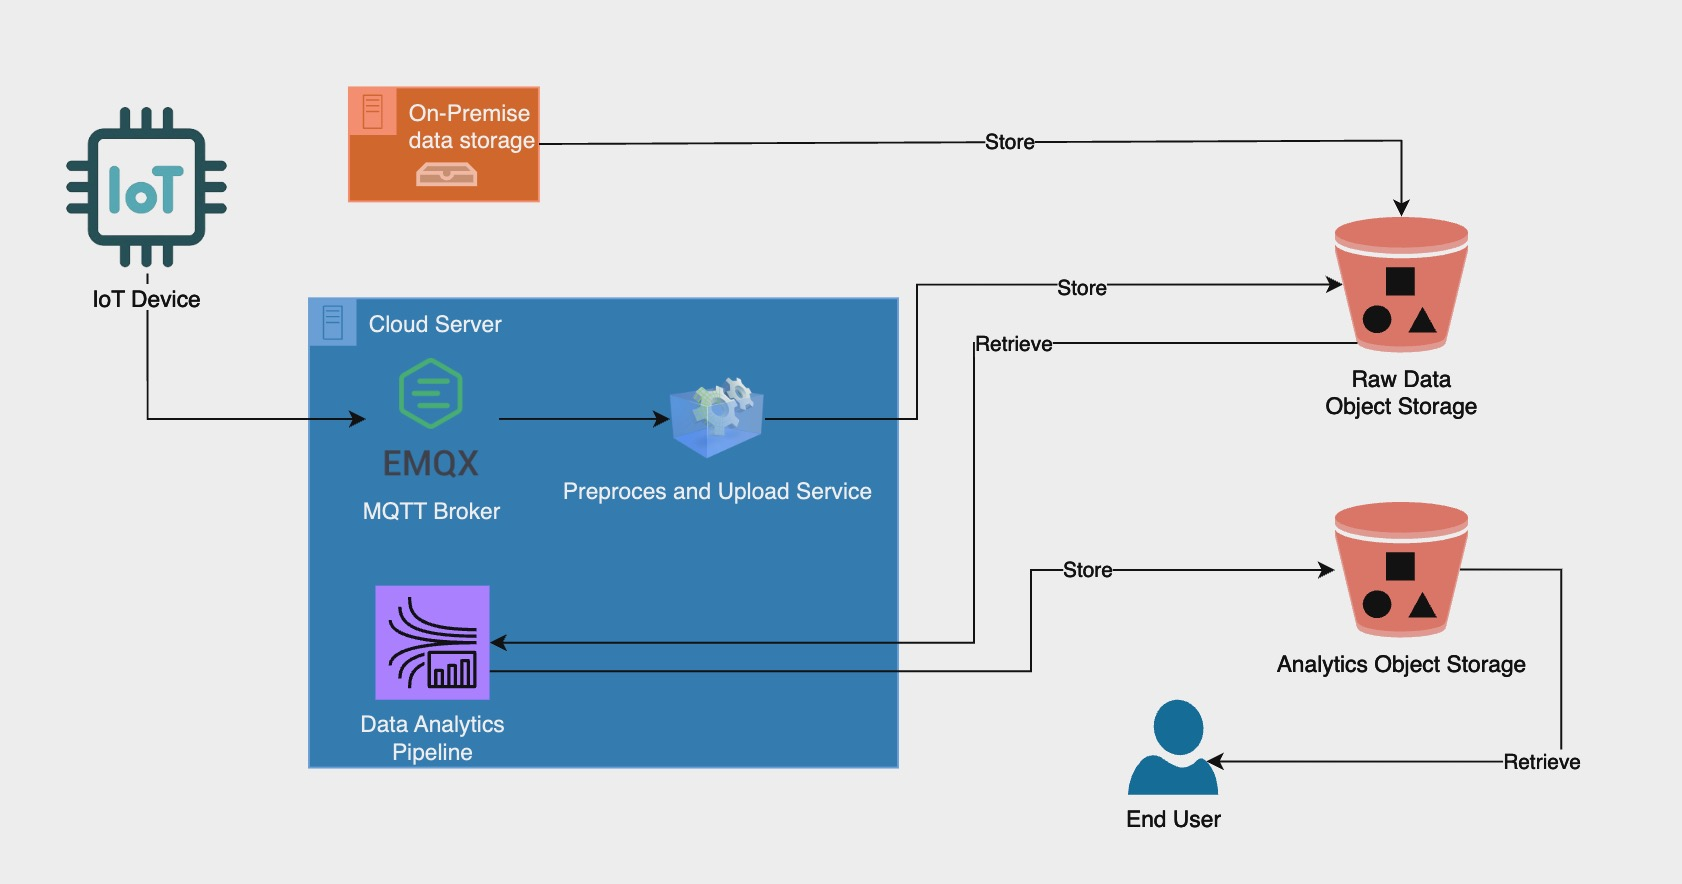
\includegraphics[width=1\textwidth]{architecture.png}
    \caption{Architecture of the proposed solution}
\end{figure}

The proposed solution's architecture consists of a composition of loosely coupled microservices that work together to collect, process, and store data. The architecture is divided into three layers: the data collection layer, the data storage layer and the data analysis layer. Each layer plays a specific role in the overall system, ensuring scalability, flexibility, and resilience.

\subsection{Data Collection Layer}

The data collection layer is responsible for gathering data from IoT devices and archived data. 

\subsection{Data Collection from IoT Devices}

The data collection from IoT devices utilizes the MQTT protocol, a lightweight messaging protocol designed for devices with low bandwidth and high latency. MQTT operates on a publish-subscribe model, where devices publish messages to a broker, which then forwards the messages to subscribers. This protocol is ideal for IoT devices due to its simplicity, ease of implementation, and reliability, with support for different quality of service (QoS) levels to ensure message delivery.

In our scenario, a large number of IoT devices publish data to the cloud. Each device publishes data on a specific topic managed by a cloud-based broker. The data is sent in JSON format, with each message containing a timestamp and a set of key-value pairs representing the data. Once the data is published to the broker, it undergoes preprocessing before being stored in object storage. This preprocessing involves parsing the JSON data, extracting the timestamp and key-value pairs, and converting the data to CSV format. The CSV format was chosen for its simplicity and compatibility with common data processing tools and libraries as well as its reduced verbosity compared to JSON. The preprocessed data is then stored in object storage, making it accessible to the data processing pipeline.


\subsection{Data Collection from Archived Data}
The data collection from archived data is done by uploading files from on-premises to the cloud via a simple script that leverages cloud API. The files, which are already in CSV format, are uploaded to the object storage, where they can be accessed by the data processing pipeline. The files contain historical data that have been collected over time in several different scenarios.

\subsection{Data Storage Layer}

The data storage layer is responsible for storing the raw CSV data and making it accessible to the data processing pipeline. This layer utilizes cloud-based object storage for scalability and durability. The data, always stored in CSV format, is uploaded to the object storage by the data collection layer and accessed by the data analysis layer.
Once the analysis is done, the results are stored in a separate object storage bucket, making them accessible to other services or users.
Object storage provides a reliable and cost-effective solution for storing large amounts of data, with built-in redundancy and scalability features.

\subsection{Data Analysis Layer}

The data analysis layer is responsible for analyzing the collected data and generating insights. This layer consists of several services that retrieve the preprocessed data from the object storage and perform various analytical tasks. The data, initially preprocessed and stored in CSV format, is accessed directly from the object storage by the microservices.

Once the data is retrieved, the microservices perform advanced analytics and machine learning tasks using custom algorithms tailored to specific requirements. These analytical processes transform the raw data into valuable insights, enabling more informed decision-making and a deeper understanding of the underlying patterns and trends in the collected data.
Right after the analysis is done, the results are stored in a separate object storage bucket, making them accessible to other services or users.

\subsection{Cloud Server vs. SaaS Solutions}

The choice of using a cloud server to host both the MQTT broker and the data analytics pipeline provides several advantages over SaaS solutions. While SaaS architectures have been considered, a cloud server offers more flexibility and control over the infrastructure, which is crucial for custom configurations and dependencies required by the data analytics pipeline. It is also more cost-effective for long-term projects, as SaaS solutions typically incur significant monthly fees. A cloud server allows better control over costs, with the trade-off being the need to manage infrastructure and security patches.

Furthermore, this solution is seamlessly implementable with any cloud provider since it doesn't rely on specific services unique to a particular provider. This cloud-agnostic approach allows users to choose the cloud provider that best fits their needs without altering the solution's architecture. Additionally, even though the MQTT broker and the data analytics pipeline are hosted on the same server, they remain independent, respecting the principles of a microservices architecture.

In summary, this architecture provides a robust, scalable, and flexible solution for data collection, processing, and storage, with the added benefit of being cloud-agnostic and cost-effective for long-term deployments.

\section{Test Implementation}

In this section, the base implementation of the proposed solution is presented. The implementation is divided into two main components: the data collection component and the data analysis component. The data collection component is responsible for collecting data from IoT devices and archived data, while the data analysis component is responsible for processing and analyzing the collected data.

\subsection{Data Collection Component}

The data collection component is responsible for collecting data from IoT devices and archived data. This component consists of three main parts: the MQTT broker, the preprocessing pipeline and the data upload script.

\subsubsection{MQTT Broker}
MQTT broker is a lightweight messaging broker that implements the MQTT protocol. The broker is responsible for receiving messages from IoT devices and forwarding them to subscribers. The broker is hosted on a cloud server and is accessible to all IoT devices connected to the network. The broker is configured to use a specific topic for each device, ensuring that messages are delivered to the correct destination. 
The chosen MQTT broker for the test implementation is \href{https://www.emqx.io/}{EMQX}\footcite{site:emqx}, whose pros and cons have been discussed in \ref{emqx}.
Once the broker have been installed and configured in the cloud server, it was tested by connecting some simulated IoT devices and sending messages to the broker. The messages were successfully received by the broker and forwarded to the subscriber, demonstrating the broker's functionality.
The IoT devices used in the test were simulated using the \href{https://mqttx.app/}{MQTTX}\footcite{site:mqttx} client, analyzed in \ref{mqttx}. This MQTT client allows users to simulate IoT devices and publish messages to an MQTT broker. The devices were configured to publish messages to the broker using a specific topic, with each message containing a timestamp and a set of key-value pairs representing the data.

\subsubsection{Preprocessing pipeline}
The preprocessing pipeline is responsible for parsing the JSON data received from the MQTT broker, extracting the timestamp and key-value pairs, and converting the data to CSV format. The pipeline is implemented as a Python script that subscribes to the MQTT broker, receives messages, and preprocesses the data. The script uses the \href{https://pypi.org/project/paho-mqtt/}{Paho MQTT}\footcite{site:paho-mqtt} client library to connect to the broker and receive messages. Once the data is received, it is parsed, and the timestamp and key-value pairs are extracted. The data is then converted to CSV format and stored in object storage. The preprocessing pipeline ensures that the data is in a suitable format for further analysis and processing. The script was tested by connecting it to the MQTT broker and receiving messages from the simulated IoT devices. The messages were successfully parsed, and the data was converted to CSV format, demonstrating the pipeline's functionality.

\subsubsection{Data Upload Script}
The data upload script is responsible for uploading archived data from on-premises to the cloud. The script is implemented as a Python script that uses the cloud provider's API to upload files to object storage. The files contain historical data that have been collected over time in many different scenarios. The script reads the files from a local directory, uploads them to object storage, and makes them accessible to the data processing pipeline. In this scenario the files are already stored in CSV format, making them suitable for direct upload to object storage. The script was tested by uploading several sample files to object storage and verifying that the files were successfully uploaded to the right directory and accessible to the data processing pipeline. 


\subsection{Data Analysis Component}
The data analysis component is responsible for processing and analyzing the collected data. This component can consist of one or more data analytics scripts based on the requirements of the project. Each of the scripts needs to retrieve the correct data from the object storage, perform the required analysis, and store the results in a separate object storage bucket. In the case more than one file needs to be retrieved from storage, the scripts need to manage the data retrieval and processing in parallel to optimize performance and resource usage. The scripts can be implemented in any programming language that supports the required data processing and analysis tasks, such as Python or R. The choice of language depends on the specific requirements of the project and the availability of libraries and tools for data processing and analysis.
This component was tested by implementing a simple data analysis script that retrieves the preprocessed data from object storage, calculates simple statistics, and stores the results in a separate object storage bucket. The script was implemented in Python using various Python libraries such as Pandas and NumPy for data manipulation and analysis. The script was tested by retrieving the preprocessed data from object storage, calculating the statistics, and storing the results in a separate object storage bucket. The results were successfully stored, demonstrating the functionality of the data analysis component.
Once the analytics are uploaded they can be accessed via a web interface or a REST API, depending on the requirements of the project. The results can be visualized using various data visualization tools such as Matplotlib, Plotly, or Tableau, providing insights into the underlying patterns and trends in the collected data.